%% ID: bomb_ship
%% TITLE: Targetting a Bomb
%% TYPE: question
%% QUESTIONTYPE: numerical
%% CONCEPTS: energy, eq_of_motions_diff, forces, newtonii
%% VIDEOS: 
%% LEVEL: 3
%% TOPIC: mechanics/kinematics
%% ORDER: 8


\begin{problem}[HSC1950MIIIQ5a] % imperial units to metric units - numbers may need tweaking
{\exposition{An aeroplane is flying on a straight horizontal course at a speed of \quantity{200}{km h\sup{-1}} at a height of \quantity{100}{m} above the top of the funnel of a ship which is at rest.  A small bomb is released from the aeroplane so that it enters the funnel, which is vertical and of diameter \quantity{7}{m}.} \question {Find the greatest depth below its top at which the funnel can be hit by the bomb.}}
{\textit{Adapted with permission from UCLES, Higher School Certificate Mathematics, Paper 3, Question 5.}}
{
As always, drawing a diagram should be the first step. Figure \ref{fig:Kinematics_planebomb} is an example, showing the bomb with its initial velocity \vari{u} in the x direction:
\begin{figure}[h]
\centering
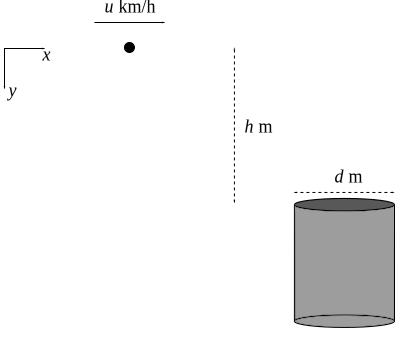
\includegraphics[width=9cm]{Kinematics_planebomb}
\caption{}
\label{fig:Kinematics_planebomb}
\end{figure}
\\
First, calculate the velocity of the bomb in the $y$ direction when it reaches the far left end of the funnel (obviously it needs to enter the funnel there to go as far as possible downwards). You can do this with SUVAT but it is faster to conserve energy:
\begin{align*}
mgh&=\frac{1}{2}mv_y^2 \\
\Rightarrow v_y&=\sqrt{2gh}
\end{align*}
Then we can say the distance down the tube \vari{\Delta y} the bomb will fall is 
\begin{align*}
\Delta y&=v_yt+\frac{1}{2}gt^2
\end{align*}
where \vari{t} is the time taken for the bomb to reach the other side of the funnel, and is given by 
\begin{align*}
t=\frac{d}{v_x}=\frac{d}{u}
\end{align*}
So the distance becomes
\begin{align*}
\Delta y&=\frac{d}{u}\sqrt{2gh}+\frac{gd^2}{2u^2} \\
&=5.66\textrm{ m}
\end{align*}
\answer{The greatest depth below the top of the funnel at which the bomb can hit the side of the funnel is \quantity{5.7}{m} .}

Notice how if you had just assumed the velocity in the $y$ direction was constant while the bomb was in the funnel, you would not have had the second term in the expression for $\Delta y$. In fact, this second term only contributes about $1\%$ of the answer so that would have been a reasonable approximation. 
}
\end{problem}